% -*- compile-command: "make slides.pdf" -*-
\documentclass{beamer}
\usepackage{tikz}
\usepackage[all]{xy}
\usepackage{amsmath,amssymb}
\usepackage{hyperref}
\usepackage{graphicx}
\usepackage{algorithmic}
\usepackage{multirow}

\DeclareMathOperator*{\argmin}{arg\,min}
\DeclareMathOperator*{\Lik}{Lik}
\DeclareMathOperator*{\PoissonLoss}{PoissonLoss}
\DeclareMathOperator*{\Peaks}{Peaks}
\DeclareMathOperator*{\Segments}{Segments}
\DeclareMathOperator*{\argmax}{arg\,max}
\DeclareMathOperator*{\maximize}{maximize}
\DeclareMathOperator*{\minimize}{minimize}
\newcommand{\sign}{\operatorname{sign}}
\newcommand{\RR}{\mathbb R}
\newcommand{\ZZ}{\mathbb Z}
\newcommand{\NN}{\mathbb N}

% Set transparency of non-highlighted sections in the table of
% contents slide.
\setbeamertemplate{section in toc shaded}[default][100]
\AtBeginSection[]
{
  \setbeamercolor{section in toc}{fg=red} 
  \setbeamercolor{section in toc shaded}{fg=black} 
  \begin{frame}
    \tableofcontents[currentsection]
  \end{frame}
}

\begin{document}

\title{Labeled Optimal Partitioning}

\author{
  Toby Dylan Hocking\\
  toby.hocking@nau.edu\\
  joint work with Anuraag Srivastava}

%c\date{6 June 2020}

\maketitle

\section{Introduction: supervised changepoint detection for cancer diagnosis with DNA copy number data}

\begin{frame}
  \frametitle{Cancer cells show chromosomal copy number alterations}
  Spectral karyotypes show the number of copies of the sex chromosomes
  (X,Y) and autosomes (1-22). 

  Source: Alberts \emph{et al.} 2002.
\vskip 0.1in
  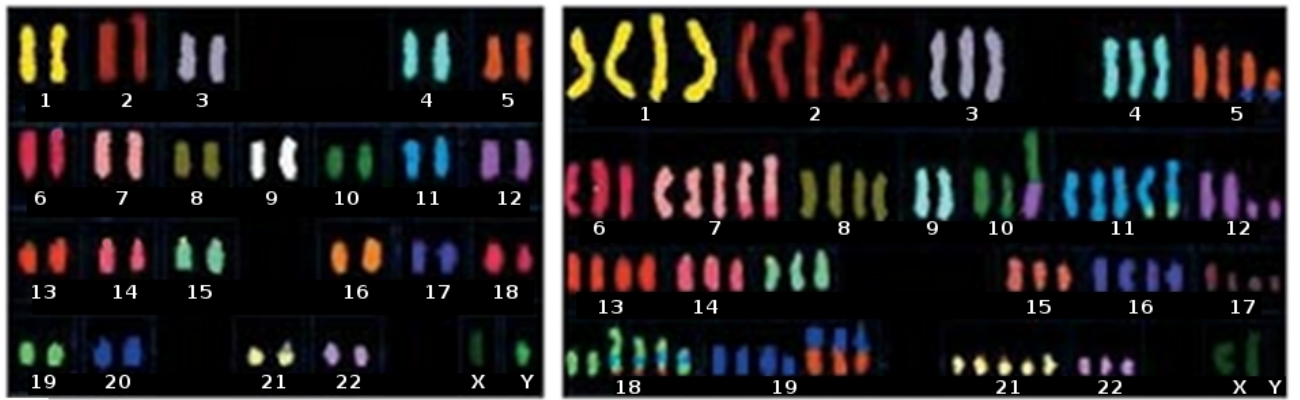
\includegraphics[width=\textwidth]{Karyo-both}
\vskip 0.1in
  \begin{minipage}{0.4\linewidth}
    Normal cell with 2 copies of each autosome.
  \end{minipage}
\hskip 0.1\linewidth
  \begin{minipage}{0.4\linewidth}
Cancer cell with many copy number alterations.
  \end{minipage}
\end{frame}

\begin{frame}
  \frametitle{DNA copy number profiles from neuroblastoma patients with or without relapse}

  \hspace*{-1cm}
  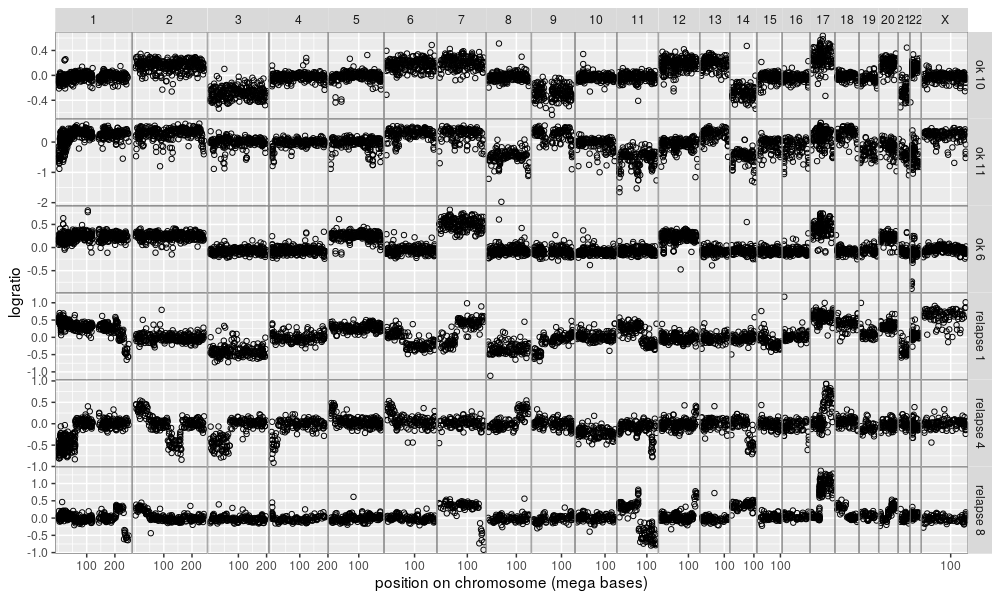
\includegraphics[width=1.15\textwidth]{figure-neuroblastoma-clinical}
  
\end{frame}

\begin{frame}
  \frametitle{Previous work: SegAnnDB interactive machine learning
    system}

  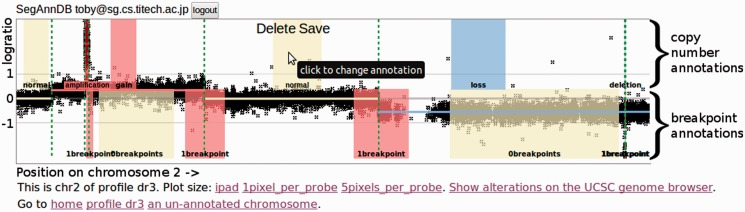
\includegraphics[width=\textwidth]{screenshot-SegAnnDB-figure-1}

  Hocking \emph{et al.}, 2014. 

  \begin{itemize}
  \item User uploads noisy data sets for machine learning analysis.
  \item User can provide labels which indicate presence(1) or
    absence(0) of changepoints in specific regions of data sets.
  \item Classic optimal changepoint model (max penalized Gaussian
    likelihood) used if it has zero label errors. OPART algorithm,
    Jackson \emph{et al.}, 2005. FPOP algorithm, Maidstone \emph{et
      al.}, 2016. 
  \item Label-aware SegAnnot algorithm used otherwise (Hocking and
    Rigaill, 2012). Always zero train label errors, but never predicts
    any changepoints outside of positive(1) labels.
  \end{itemize}
  
\end{frame}

\begin{frame}
  \frametitle{Example noisy data sequence}

  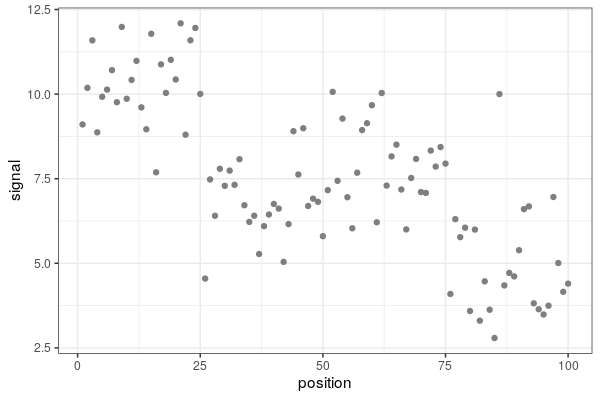
\includegraphics[width=\textwidth]{figure-baselines-data} 
  
\end{frame}

\begin{frame}
  \frametitle{Example noisy data sequence with labels}

  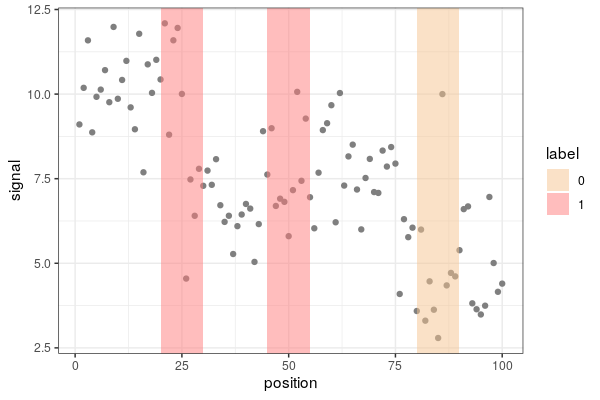
\includegraphics[width=\textwidth]{figure-baselines-labels}  
  
\end{frame}


\begin{frame}
  \frametitle{OPART with penalty $\lambda=1000$ (ignores labels)}
  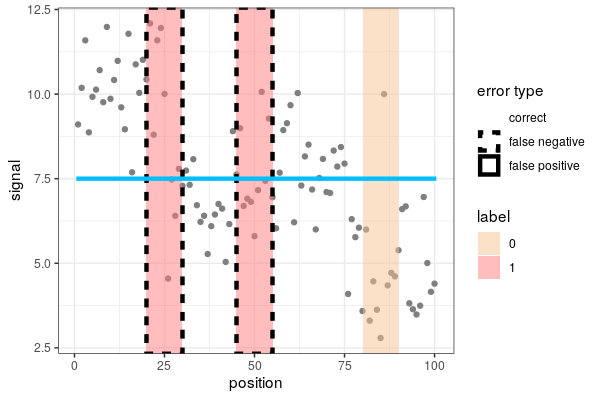
\includegraphics[width=\textwidth]{figure-baselines-penalty=1000.png}
\end{frame}


\begin{frame}
  \frametitle{OPART with penalty $\lambda=100$ (ignores labels)}
  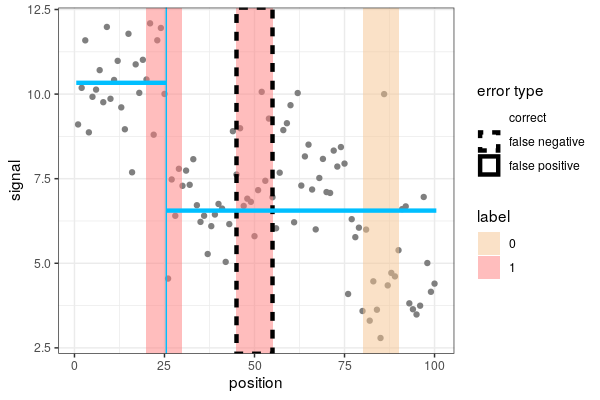
\includegraphics[width=\textwidth]{figure-baselines-penalty=100.png}
\end{frame}


\begin{frame}
  \frametitle{OPART with penalty $\lambda=20$ (ignores labels)}
  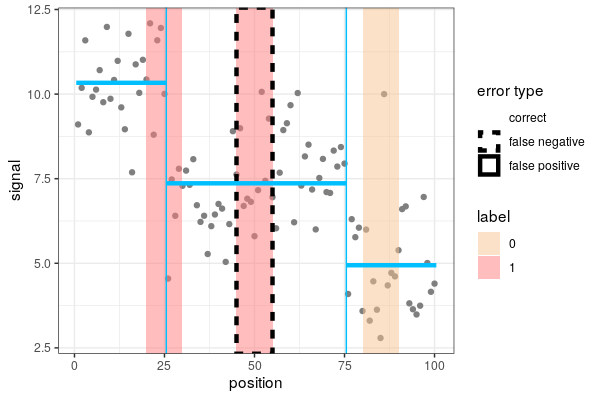
\includegraphics[width=\textwidth]{figure-baselines-penalty=20.png}
\end{frame}


\begin{frame}
  \frametitle{OPART with penalty $\lambda=15$ (ignores labels)}
  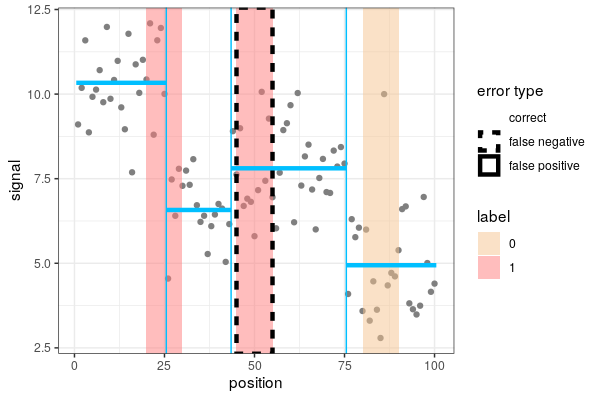
\includegraphics[width=\textwidth]{figure-baselines-penalty=15.png}
\end{frame}


\begin{frame}
  \frametitle{OPART with penalty $\lambda=10$ (ignores labels)}
  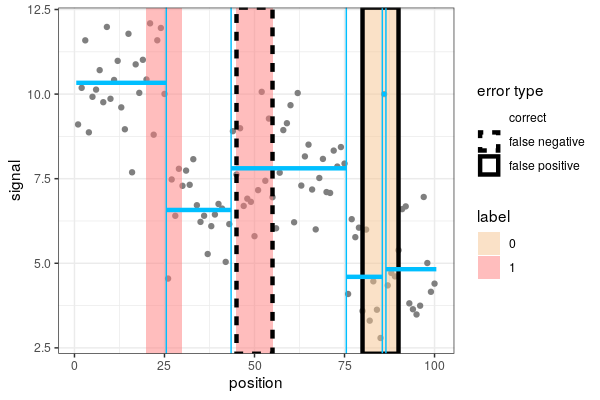
\includegraphics[width=\textwidth]{figure-baselines-penalty=10.png}
\end{frame}


\begin{frame}
  \frametitle{OPART with penalty $\lambda=5$ (ignores labels)}
  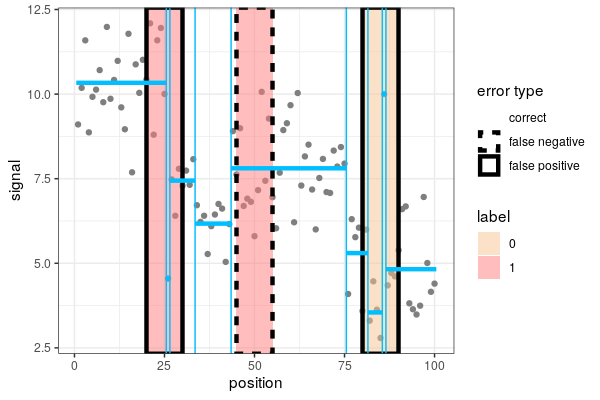
\includegraphics[width=\textwidth]{figure-baselines-penalty=5.png}
\end{frame}


\begin{frame}
  \frametitle{OPART with penalty $\lambda=4$ (ignores labels)}
  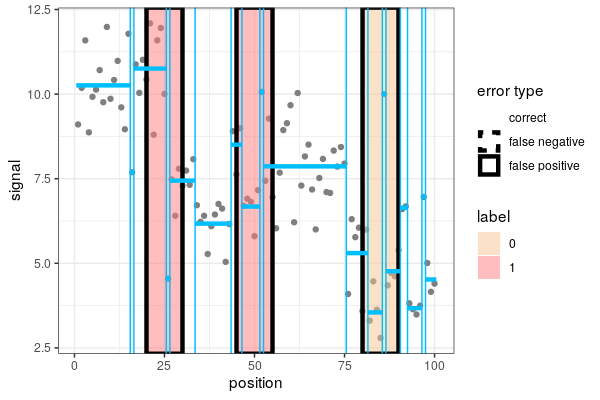
\includegraphics[width=\textwidth]{figure-baselines-penalty=4.png}
\end{frame}


\begin{frame}
  \frametitle{OPART with penalty $\lambda=0$ (ignores labels)}
  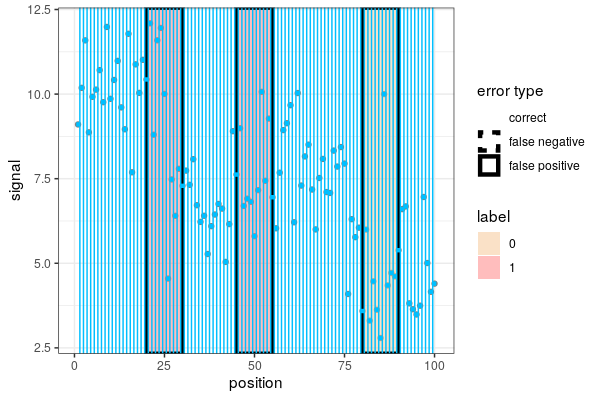
\includegraphics[width=\textwidth]{figure-baselines-penalty=0.png}
\end{frame}


\begin{frame}
  \frametitle{SegAnnot (no changes in unlabeled regions)}
  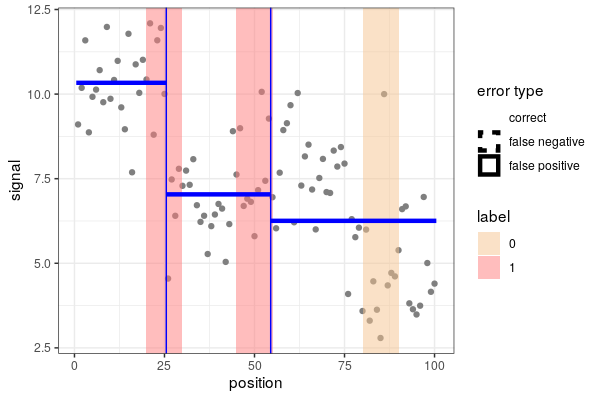
\includegraphics[width=\textwidth]{figure-baselines-penalty=Inf.png}
\end{frame}


\section{Labeled Optimal Partitioning (LOPART)}

\begin{frame}
  \frametitle{Baseline/previous OPART algorithm}

  Assume
  \begin{itemize}
  \item $\mathbf x = [ x_1 \cdots x_N ]$ is the sequence of $N$ data,
  \item $\ell$ is a loss function (e.g. square loss),
  \item $I$ the indicator function counts the number of changes,
  \item $\lambda$ is a non-negative penalty (larger for fewer changes).
  \end{itemize}
  Then the problem and algorithm are
  \begin{eqnarray*}
    \label{eq:op}
    \hat C_N &=& \min_{\mathbf m\in \mathbb R^N}
                 \sum_{i=1}^N \ell(m_i, x_i) + 
                 \lambda \sum_{i=1}^{N-1} I[m_i \neq m_{i+1}].\\
             &=& \min_{\tau\in \{0, 1, \dots, N-1\} }
                 \hat C_\tau +
                 \lambda +
                 L(\tau+1, N, \mathbf x).
                 \label{eq:op-update}
  \end{eqnarray*}
  where
  \begin{itemize}
  \item $\tau$ is the last changepoint optimization variable,
  \item $\hat C_\tau$ is the optimal cost computed in previous iteration $\tau$,
  \item $L$ is the cost of the last segment.
  \end{itemize}

\end{frame}

\section{LOPART Demo}

% from https://tex.stackexchange.com/questions/160825/modifying-margins-for-one-slide
\newcommand\Wider[2][3cm]{%
\makebox[\linewidth][c]{%
  \begin{minipage}{\dimexpr\textwidth+#1\relax}
  \raggedright#2
  \end{minipage}%
  }%
}

\input{figure-candidates}

\section{Results and Discussion}

\begin{frame}
  \frametitle{Empirical time complexity (labels)}
  % Created by tikzDevice version 0.12.3 on 2020-10-15 16:28:37
% !TEX encoding = UTF-8 Unicode
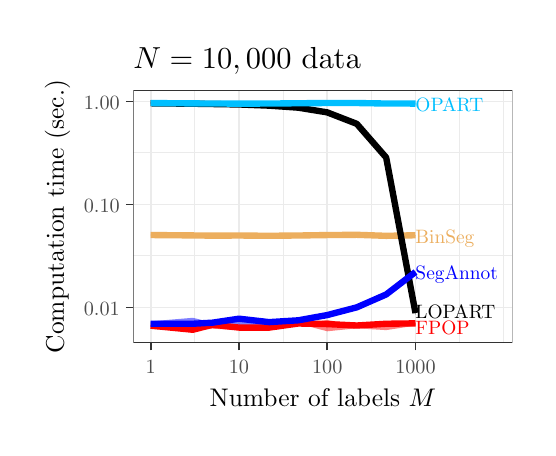
\begin{tikzpicture}[x=1pt,y=1pt]
\definecolor{fillColor}{RGB}{255,255,255}
\path[use as bounding box,fill=fillColor,fill opacity=0.00] (0,0) rectangle (180.67,144.54);
\begin{scope}
\path[clip] (  0.00,  0.00) rectangle (180.67,144.54);
\definecolor{drawColor}{RGB}{255,255,255}
\definecolor{fillColor}{RGB}{255,255,255}

\path[draw=drawColor,line width= 0.6pt,line join=round,line cap=round,fill=fillColor] ( -0.00,  0.00) rectangle (180.67,144.54);
\end{scope}
\begin{scope}
\path[clip] ( 38.23, 30.69) rectangle (175.17,121.88);
\definecolor{fillColor}{RGB}{255,255,255}

\path[fill=fillColor] ( 38.23, 30.69) rectangle (175.17,121.88);
\definecolor{drawColor}{gray}{0.92}

\path[draw=drawColor,line width= 0.3pt,line join=round] ( 38.23, 62.09) --
	(175.17, 62.09);

\path[draw=drawColor,line width= 0.3pt,line join=round] ( 38.23, 99.30) --
	(175.17, 99.30);

\path[draw=drawColor,line width= 0.3pt,line join=round] ( 60.40, 30.69) --
	( 60.40,121.88);

\path[draw=drawColor,line width= 0.3pt,line join=round] ( 92.30, 30.69) --
	( 92.30,121.88);

\path[draw=drawColor,line width= 0.3pt,line join=round] (124.20, 30.69) --
	(124.20,121.88);

\path[draw=drawColor,line width= 0.3pt,line join=round] (156.09, 30.69) --
	(156.09,121.88);

\path[draw=drawColor,line width= 0.3pt,line join=round] (172.04, 30.69) --
	(172.04,121.88);

\path[draw=drawColor,line width= 0.6pt,line join=round] ( 38.23, 43.48) --
	(175.17, 43.48);

\path[draw=drawColor,line width= 0.6pt,line join=round] ( 38.23, 80.69) --
	(175.17, 80.69);

\path[draw=drawColor,line width= 0.6pt,line join=round] ( 38.23,117.91) --
	(175.17,117.91);

\path[draw=drawColor,line width= 0.6pt,line join=round] ( 44.45, 30.69) --
	( 44.45,121.88);

\path[draw=drawColor,line width= 0.6pt,line join=round] ( 76.35, 30.69) --
	( 76.35,121.88);

\path[draw=drawColor,line width= 0.6pt,line join=round] (108.25, 30.69) --
	(108.25,121.88);

\path[draw=drawColor,line width= 0.6pt,line join=round] (140.14, 30.69) --
	(140.14,121.88);
\definecolor{fillColor}{RGB}{236,174,94}

\path[fill=fillColor,fill opacity=0.50] ( 44.45, 69.85) --
	( 59.67, 69.52) --
	( 66.75, 69.51) --
	( 76.35, 69.52) --
	( 87.27, 69.64) --
	( 97.79, 69.57) --
	(108.25, 69.60) --
	(118.92, 69.69) --
	(129.54, 69.99) --
	(140.14, 69.67) --
	(140.14, 69.32) --
	(129.54, 69.20) --
	(118.92, 69.57) --
	(108.25, 69.57) --
	( 97.79, 69.23) --
	( 87.27, 69.20) --
	( 76.35, 69.14) --
	( 66.75, 69.23) --
	( 59.67, 69.37) --
	( 44.45, 69.44) --
	cycle;

\path[] ( 44.45, 69.85) --
	( 59.67, 69.52) --
	( 66.75, 69.51) --
	( 76.35, 69.52) --
	( 87.27, 69.64) --
	( 97.79, 69.57) --
	(108.25, 69.60) --
	(118.92, 69.69) --
	(129.54, 69.99) --
	(140.14, 69.67);

\path[] (140.14, 69.32) --
	(129.54, 69.20) --
	(118.92, 69.57) --
	(108.25, 69.57) --
	( 97.79, 69.23) --
	( 87.27, 69.20) --
	( 76.35, 69.14) --
	( 66.75, 69.23) --
	( 59.67, 69.37) --
	( 44.45, 69.44);
\definecolor{fillColor}{RGB}{255,0,0}

\path[fill=fillColor,fill opacity=0.50] ( 44.45, 37.23) --
	( 59.67, 36.45) --
	( 66.75, 37.65) --
	( 76.35, 36.77) --
	( 87.27, 37.30) --
	( 97.79, 37.85) --
	(108.25, 38.91) --
	(118.92, 37.06) --
	(129.54, 37.90) --
	(140.14, 38.38) --
	(140.14, 36.88) --
	(129.54, 35.25) --
	(118.92, 35.91) --
	(108.25, 34.83) --
	( 97.79, 37.56) --
	( 87.27, 35.14) --
	( 76.35, 35.27) --
	( 66.75, 35.77) --
	( 59.67, 35.06) --
	( 44.45, 35.71) --
	cycle;

\path[] ( 44.45, 37.23) --
	( 59.67, 36.45) --
	( 66.75, 37.65) --
	( 76.35, 36.77) --
	( 87.27, 37.30) --
	( 97.79, 37.85) --
	(108.25, 38.91) --
	(118.92, 37.06) --
	(129.54, 37.90) --
	(140.14, 38.38);

\path[] (140.14, 36.88) --
	(129.54, 35.25) --
	(118.92, 35.91) --
	(108.25, 34.83) --
	( 97.79, 37.56) --
	( 87.27, 35.14) --
	( 76.35, 35.27) --
	( 66.75, 35.77) --
	( 59.67, 35.06) --
	( 44.45, 35.71);
\definecolor{fillColor}{RGB}{0,0,0}

\path[fill=fillColor,fill opacity=0.50] ( 44.45,117.53) --
	( 59.67,117.05) --
	( 66.75,117.04) --
	( 76.35,116.84) --
	( 87.27,116.37) --
	( 97.79,116.50) --
	(108.25,113.98) --
	(118.92,109.80) --
	(129.54, 97.82) --
	(140.14, 43.13) --
	(140.14, 40.74) --
	(129.54, 97.47) --
	(118.92,109.70) --
	(108.25,113.88) --
	( 97.79,115.59) --
	( 87.27,116.35) --
	( 76.35,116.78) --
	( 66.75,116.93) --
	( 59.67,117.00) --
	( 44.45,117.11) --
	cycle;

\path[] ( 44.45,117.53) --
	( 59.67,117.05) --
	( 66.75,117.04) --
	( 76.35,116.84) --
	( 87.27,116.37) --
	( 97.79,116.50) --
	(108.25,113.98) --
	(118.92,109.80) --
	(129.54, 97.82) --
	(140.14, 43.13);

\path[] (140.14, 40.74) --
	(129.54, 97.47) --
	(118.92,109.70) --
	(108.25,113.88) --
	( 97.79,115.59) --
	( 87.27,116.35) --
	( 76.35,116.78) --
	( 66.75,116.93) --
	( 59.67,117.00) --
	( 44.45,117.11);
\definecolor{fillColor}{RGB}{0,191,255}

\path[fill=fillColor,fill opacity=0.50] ( 44.45,117.43) --
	( 59.67,117.24) --
	( 66.75,117.18) --
	( 76.35,117.13) --
	( 87.27,117.12) --
	( 97.79,117.74) --
	(108.25,117.33) --
	(118.92,117.58) --
	(129.54,117.30) --
	(140.14,117.25) --
	(140.14,117.10) --
	(129.54,117.11) --
	(118.92,117.26) --
	(108.25,117.28) --
	( 97.79,117.10) --
	( 87.27,117.11) --
	( 76.35,117.10) --
	( 66.75,117.10) --
	( 59.67,117.14) --
	( 44.45,117.24) --
	cycle;

\path[] ( 44.45,117.43) --
	( 59.67,117.24) --
	( 66.75,117.18) --
	( 76.35,117.13) --
	( 87.27,117.12) --
	( 97.79,117.74) --
	(108.25,117.33) --
	(118.92,117.58) --
	(129.54,117.30) --
	(140.14,117.25);

\path[] (140.14,117.10) --
	(129.54,117.11) --
	(118.92,117.26) --
	(108.25,117.28) --
	( 97.79,117.10) --
	( 87.27,117.11) --
	( 76.35,117.10) --
	( 66.75,117.10) --
	( 59.67,117.14) --
	( 44.45,117.24);
\definecolor{fillColor}{RGB}{0,0,255}

\path[fill=fillColor,fill opacity=0.50] ( 44.45, 38.43) --
	( 59.67, 39.70) --
	( 66.75, 38.01) --
	( 76.35, 39.40) --
	( 87.27, 38.41) --
	( 97.79, 39.62) --
	(108.25, 40.88) --
	(118.92, 44.28) --
	(129.54, 48.28) --
	(140.14, 56.49) --
	(140.14, 56.03) --
	(129.54, 48.03) --
	(118.92, 43.25) --
	(108.25, 40.67) --
	( 97.79, 38.70) --
	( 87.27, 37.20) --
	( 76.35, 36.89) --
	( 66.75, 37.25) --
	( 59.67, 36.20) --
	( 44.45, 36.36) --
	cycle;

\path[] ( 44.45, 38.43) --
	( 59.67, 39.70) --
	( 66.75, 38.01) --
	( 76.35, 39.40) --
	( 87.27, 38.41) --
	( 97.79, 39.62) --
	(108.25, 40.88) --
	(118.92, 44.28) --
	(129.54, 48.28) --
	(140.14, 56.49);

\path[] (140.14, 56.03) --
	(129.54, 48.03) --
	(118.92, 43.25) --
	(108.25, 40.67) --
	( 97.79, 38.70) --
	( 87.27, 37.20) --
	( 76.35, 36.89) --
	( 66.75, 37.25) --
	( 59.67, 36.20) --
	( 44.45, 36.36);
\definecolor{drawColor}{RGB}{236,174,94}

\path[draw=drawColor,line width= 2.3pt,line join=round] ( 44.45, 69.61) --
	( 59.67, 69.47) --
	( 66.75, 69.38) --
	( 76.35, 69.43) --
	( 87.27, 69.34) --
	( 97.79, 69.44) --
	(108.25, 69.60) --
	(118.92, 69.69) --
	(129.54, 69.32) --
	(140.14, 69.53);
\definecolor{drawColor}{RGB}{255,0,0}

\path[draw=drawColor,line width= 2.3pt,line join=round] ( 44.45, 36.86) --
	( 59.67, 35.38) --
	( 66.75, 37.20) --
	( 76.35, 36.17) --
	( 87.27, 36.16) --
	( 97.79, 37.64) --
	(108.25, 37.43) --
	(118.92, 36.92) --
	(129.54, 37.55) --
	(140.14, 37.70);
\definecolor{drawColor}{RGB}{0,0,0}

\path[draw=drawColor,line width= 2.3pt,line join=round] ( 44.45,117.21) --
	( 59.67,117.05) --
	( 66.75,116.94) --
	( 76.35,116.79) --
	( 87.27,116.36) --
	( 97.79,115.63) --
	(108.25,113.93) --
	(118.92,109.79) --
	(129.54, 97.62) --
	(140.14, 41.41);
\definecolor{drawColor}{RGB}{0,191,255}

\path[draw=drawColor,line width= 2.3pt,line join=round] ( 44.45,117.30) --
	( 59.67,117.18) --
	( 66.75,117.13) --
	( 76.35,117.10) --
	( 87.27,117.12) --
	( 97.79,117.23) --
	(108.25,117.31) --
	(118.92,117.31) --
	(129.54,117.13) --
	(140.14,117.11);
\definecolor{drawColor}{RGB}{0,0,255}

\path[draw=drawColor,line width= 2.3pt,line join=round] ( 44.45, 37.56) --
	( 59.67, 37.55) --
	( 66.75, 37.94) --
	( 76.35, 39.38) --
	( 87.27, 38.14) --
	( 97.79, 38.80) --
	(108.25, 40.69) --
	(118.92, 43.48) --
	(129.54, 48.13) --
	(140.14, 56.26);
\end{scope}
\begin{scope}
\path[clip] ( 38.23, 30.69) rectangle (175.17,121.88);
\definecolor{drawColor}{RGB}{255,0,0}

\node[text=drawColor,anchor=base west,inner sep=0pt, outer sep=0pt, scale=  0.70] at (140.14, 33.77) {FPOP};
\definecolor{drawColor}{RGB}{0,0,0}

\node[text=drawColor,anchor=base west,inner sep=0pt, outer sep=0pt, scale=  0.70] at (140.14, 39.56) {LOPART};
\definecolor{drawColor}{RGB}{0,0,255}

\node[text=drawColor,anchor=base west,inner sep=0pt, outer sep=0pt, scale=  0.70] at (140.14, 53.37) {SegAnnot};
\definecolor{drawColor}{RGB}{236,174,94}

\node[text=drawColor,anchor=base west,inner sep=0pt, outer sep=0pt, scale=  0.70] at (140.14, 66.63) {BinSeg};
\definecolor{drawColor}{RGB}{0,191,255}

\node[text=drawColor,anchor=base west,inner sep=0pt, outer sep=0pt, scale=  0.70] at (140.14,114.21) {OPART};
\definecolor{drawColor}{gray}{0.20}

\path[draw=drawColor,line width= 0.6pt,line join=round,line cap=round] ( 38.23, 30.69) rectangle (175.17,121.88);
\end{scope}
\begin{scope}
\path[clip] (  0.00,  0.00) rectangle (180.67,144.54);
\definecolor{drawColor}{gray}{0.30}

\node[text=drawColor,anchor=base east,inner sep=0pt, outer sep=0pt, scale=  0.73] at ( 33.28, 40.45) {0.01};

\node[text=drawColor,anchor=base east,inner sep=0pt, outer sep=0pt, scale=  0.73] at ( 33.28, 77.66) {0.10};

\node[text=drawColor,anchor=base east,inner sep=0pt, outer sep=0pt, scale=  0.73] at ( 33.28,114.88) {1.00};
\end{scope}
\begin{scope}
\path[clip] (  0.00,  0.00) rectangle (180.67,144.54);
\definecolor{drawColor}{gray}{0.20}

\path[draw=drawColor,line width= 0.6pt,line join=round] ( 35.48, 43.48) --
	( 38.23, 43.48);

\path[draw=drawColor,line width= 0.6pt,line join=round] ( 35.48, 80.69) --
	( 38.23, 80.69);

\path[draw=drawColor,line width= 0.6pt,line join=round] ( 35.48,117.91) --
	( 38.23,117.91);
\end{scope}
\begin{scope}
\path[clip] (  0.00,  0.00) rectangle (180.67,144.54);
\definecolor{drawColor}{gray}{0.20}

\path[draw=drawColor,line width= 0.6pt,line join=round] ( 44.45, 27.94) --
	( 44.45, 30.69);

\path[draw=drawColor,line width= 0.6pt,line join=round] ( 76.35, 27.94) --
	( 76.35, 30.69);

\path[draw=drawColor,line width= 0.6pt,line join=round] (108.25, 27.94) --
	(108.25, 30.69);

\path[draw=drawColor,line width= 0.6pt,line join=round] (140.14, 27.94) --
	(140.14, 30.69);
\end{scope}
\begin{scope}
\path[clip] (  0.00,  0.00) rectangle (180.67,144.54);
\definecolor{drawColor}{gray}{0.30}

\node[text=drawColor,anchor=base,inner sep=0pt, outer sep=0pt, scale=  0.73] at ( 44.45, 19.68) {1};

\node[text=drawColor,anchor=base,inner sep=0pt, outer sep=0pt, scale=  0.73] at ( 76.35, 19.68) {10};

\node[text=drawColor,anchor=base,inner sep=0pt, outer sep=0pt, scale=  0.73] at (108.25, 19.68) {100};

\node[text=drawColor,anchor=base,inner sep=0pt, outer sep=0pt, scale=  0.73] at (140.14, 19.68) {1000};
\end{scope}
\begin{scope}
\path[clip] (  0.00,  0.00) rectangle (180.67,144.54);
\definecolor{drawColor}{RGB}{0,0,0}

\node[text=drawColor,anchor=base,inner sep=0pt, outer sep=0pt, scale=  0.92] at (106.70,  7.64) {Number of labels $M$};
\end{scope}
\begin{scope}
\path[clip] (  0.00,  0.00) rectangle (180.67,144.54);
\definecolor{drawColor}{RGB}{0,0,0}

\node[text=drawColor,rotate= 90.00,anchor=base,inner sep=0pt, outer sep=0pt, scale=  0.92] at ( 13.08, 76.28) {Computation time (sec.)};
\end{scope}
\begin{scope}
\path[clip] (  0.00,  0.00) rectangle (180.67,144.54);
\definecolor{drawColor}{RGB}{0,0,0}

\node[text=drawColor,anchor=base west,inner sep=0pt, outer sep=0pt, scale=  1.10] at ( 38.23,129.95) {$N=10,000$ data};
\end{scope}
\end{tikzpicture}

\end{frame}

\begin{frame}
  \frametitle{Empirical time complexity (data)}
  % Created by tikzDevice version 0.12.3 on 2020-06-04 22:28:42
% !TEX encoding = UTF-8 Unicode
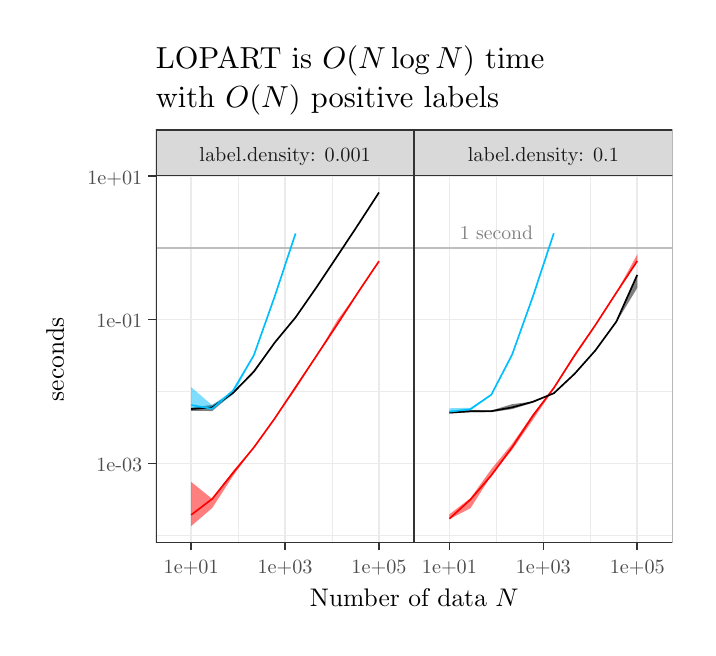
\begin{tikzpicture}[x=1pt,y=1pt]
\definecolor{fillColor}{RGB}{255,255,255}
\path[use as bounding box,fill=fillColor,fill opacity=0.00] (0,0) rectangle (238.49,216.81);
\begin{scope}
\path[clip] (  0.00,  0.00) rectangle (238.49,216.81);
\definecolor{drawColor}{RGB}{255,255,255}
\definecolor{fillColor}{RGB}{255,255,255}

\path[draw=drawColor,line width= 0.6pt,line join=round,line cap=round,fill=fillColor] (  0.00,  0.00) rectangle (238.49,216.81);
\end{scope}
\begin{scope}
\path[clip] ( 46.36, 30.69) rectangle (139.68,163.33);
\definecolor{fillColor}{RGB}{255,255,255}

\path[fill=fillColor] ( 46.36, 30.69) rectangle (139.68,163.33);
\definecolor{drawColor}{gray}{0.92}

\path[draw=drawColor,line width= 0.3pt,line join=round] ( 46.36, 33.41) --
	(139.68, 33.41);

\path[draw=drawColor,line width= 0.3pt,line join=round] ( 46.36, 85.35) --
	(139.68, 85.35);

\path[draw=drawColor,line width= 0.3pt,line join=round] ( 46.36,137.29) --
	(139.68,137.29);

\path[draw=drawColor,line width= 0.3pt,line join=round] ( 76.06, 30.69) --
	( 76.06,163.33);

\path[draw=drawColor,line width= 0.3pt,line join=round] (109.99, 30.69) --
	(109.99,163.33);

\path[draw=drawColor,line width= 0.6pt,line join=round] ( 46.36, 59.38) --
	(139.68, 59.38);

\path[draw=drawColor,line width= 0.6pt,line join=round] ( 46.36,111.32) --
	(139.68,111.32);

\path[draw=drawColor,line width= 0.6pt,line join=round] ( 46.36,163.26) --
	(139.68,163.26);

\path[draw=drawColor,line width= 0.6pt,line join=round] ( 59.09, 30.69) --
	( 59.09,163.33);

\path[draw=drawColor,line width= 0.6pt,line join=round] ( 93.02, 30.69) --
	( 93.02,163.33);

\path[draw=drawColor,line width= 0.6pt,line join=round] (126.95, 30.69) --
	(126.95,163.33);
\definecolor{drawColor}{RGB}{190,190,190}

\path[draw=drawColor,line width= 0.6pt,line join=round] ( 46.36,137.29) -- (139.68,137.29);
\definecolor{fillColor}{RGB}{255,0,0}

\path[fill=fillColor,fill opacity=0.50] ( 59.09, 52.65) --
	( 66.68, 46.53) --
	( 74.22, 56.61) --
	( 81.73, 65.18) --
	( 89.26, 75.82) --
	( 96.80, 86.94) --
	(104.33, 98.20) --
	(111.87,111.09) --
	(119.41,121.28) --
	(126.95,132.64) --
	(126.95,132.37) --
	(119.41,120.85) --
	(111.87,109.53) --
	(104.33, 98.03) --
	( 96.80, 86.08) --
	( 89.26, 75.54) --
	( 81.73, 65.09) --
	( 74.22, 54.88) --
	( 66.68, 43.24) --
	( 59.09, 36.71) --
	cycle;

\path[] ( 59.09, 52.65) --
	( 66.68, 46.53) --
	( 74.22, 56.61) --
	( 81.73, 65.18) --
	( 89.26, 75.82) --
	( 96.80, 86.94) --
	(104.33, 98.20) --
	(111.87,111.09) --
	(119.41,121.28) --
	(126.95,132.64);

\path[] (126.95,132.37) --
	(119.41,120.85) --
	(111.87,109.53) --
	(104.33, 98.03) --
	( 96.80, 86.08) --
	( 89.26, 75.54) --
	( 81.73, 65.09) --
	( 74.22, 54.88) --
	( 66.68, 43.24) --
	( 59.09, 36.71);
\definecolor{fillColor}{RGB}{0,0,0}

\path[fill=fillColor,fill opacity=0.50] ( 59.09, 79.51) --
	( 66.68, 80.51) --
	( 74.22, 84.87) --
	( 81.73, 93.02) --
	( 89.26,103.01) --
	( 96.80,112.19) --
	(104.33,122.96) --
	(111.87,134.56) --
	(119.41,145.72) --
	(126.95,157.30) --
	(126.95,157.17) --
	(119.41,145.62) --
	(111.87,134.17) --
	(104.33,122.94) --
	( 96.80,111.98) --
	( 89.26,102.82) --
	( 81.73, 92.38) --
	( 74.22, 84.63) --
	( 66.68, 78.28) --
	( 59.09, 78.36) --
	cycle;

\path[] ( 59.09, 79.51) --
	( 66.68, 80.51) --
	( 74.22, 84.87) --
	( 81.73, 93.02) --
	( 89.26,103.01) --
	( 96.80,112.19) --
	(104.33,122.96) --
	(111.87,134.56) --
	(119.41,145.72) --
	(126.95,157.30);

\path[] (126.95,157.17) --
	(119.41,145.62) --
	(111.87,134.17) --
	(104.33,122.94) --
	( 96.80,111.98) --
	( 89.26,102.82) --
	( 81.73, 92.38) --
	( 74.22, 84.63) --
	( 66.68, 78.28) --
	( 59.09, 78.36);
\definecolor{fillColor}{RGB}{0,191,255}

\path[fill=fillColor,fill opacity=0.50] ( 59.09, 86.91) --
	( 66.68, 80.35) --
	( 74.22, 85.81) --
	( 81.73, 98.65) --
	( 89.26,119.77) --
	( 96.80,142.45) --
	( 96.80,142.39) --
	( 89.26,119.65) --
	( 81.73, 98.34) --
	( 74.22, 84.16) --
	( 66.68, 78.89) --
	( 59.09, 79.24) --
	cycle;

\path[] ( 59.09, 86.91) --
	( 66.68, 80.35) --
	( 74.22, 85.81) --
	( 81.73, 98.65) --
	( 89.26,119.77) --
	( 96.80,142.45);

\path[] ( 96.80,142.39) --
	( 89.26,119.65) --
	( 81.73, 98.34) --
	( 74.22, 84.16) --
	( 66.68, 78.89) --
	( 59.09, 79.24);
\definecolor{drawColor}{RGB}{255,0,0}

\path[draw=drawColor,line width= 0.6pt,line join=round] ( 59.09, 40.76) --
	( 66.68, 46.53) --
	( 74.22, 55.97) --
	( 81.73, 65.12) --
	( 89.26, 75.57) --
	( 96.80, 86.90) --
	(104.33, 98.20) --
	(111.87,109.59) --
	(119.41,121.22) --
	(126.95,132.43);
\definecolor{drawColor}{RGB}{0,0,0}

\path[draw=drawColor,line width= 0.6pt,line join=round] ( 59.09, 79.00) --
	( 66.68, 79.58) --
	( 74.22, 84.85) --
	( 81.73, 92.50) --
	( 89.26,103.00) --
	( 96.80,112.11) --
	(104.33,122.95) --
	(111.87,134.23) --
	(119.41,145.63) --
	(126.95,157.27);
\definecolor{drawColor}{RGB}{0,191,255}

\path[draw=drawColor,line width= 0.6pt,line join=round] ( 59.09, 80.44) --
	( 66.68, 79.08) --
	( 74.22, 85.67) --
	( 81.73, 98.43) --
	( 89.26,119.68) --
	( 96.80,142.44);
\definecolor{drawColor}{gray}{0.20}

\path[draw=drawColor,line width= 0.6pt,line join=round,line cap=round] ( 46.36, 30.69) rectangle (139.68,163.33);
\end{scope}
\begin{scope}
\path[clip] (139.68, 30.69) rectangle (232.99,163.33);
\definecolor{fillColor}{RGB}{255,255,255}

\path[fill=fillColor] (139.68, 30.69) rectangle (232.99,163.33);
\definecolor{drawColor}{gray}{0.92}

\path[draw=drawColor,line width= 0.3pt,line join=round] (139.68, 33.41) --
	(232.99, 33.41);

\path[draw=drawColor,line width= 0.3pt,line join=round] (139.68, 85.35) --
	(232.99, 85.35);

\path[draw=drawColor,line width= 0.3pt,line join=round] (139.68,137.29) --
	(232.99,137.29);

\path[draw=drawColor,line width= 0.3pt,line join=round] (169.37, 30.69) --
	(169.37,163.33);

\path[draw=drawColor,line width= 0.3pt,line join=round] (203.30, 30.69) --
	(203.30,163.33);

\path[draw=drawColor,line width= 0.6pt,line join=round] (139.68, 59.38) --
	(232.99, 59.38);

\path[draw=drawColor,line width= 0.6pt,line join=round] (139.68,111.32) --
	(232.99,111.32);

\path[draw=drawColor,line width= 0.6pt,line join=round] (139.68,163.26) --
	(232.99,163.26);

\path[draw=drawColor,line width= 0.6pt,line join=round] (152.40, 30.69) --
	(152.40,163.33);

\path[draw=drawColor,line width= 0.6pt,line join=round] (186.33, 30.69) --
	(186.33,163.33);

\path[draw=drawColor,line width= 0.6pt,line join=round] (220.27, 30.69) --
	(220.27,163.33);
\definecolor{drawColor}{RGB}{190,190,190}

\path[draw=drawColor,line width= 0.6pt,line join=round] (139.68,137.29) -- (232.99,137.29);
\definecolor{drawColor}{gray}{0.50}

\node[text=drawColor,anchor=base,inner sep=0pt, outer sep=0pt, scale=  0.71] at (169.37,140.23) {1 second};
\definecolor{fillColor}{RGB}{255,0,0}

\path[fill=fillColor,fill opacity=0.50] (152.40, 40.97) --
	(159.99, 46.79) --
	(167.54, 57.28) --
	(175.04, 66.40) --
	(182.57, 77.09) --
	(190.11, 86.88) --
	(197.65, 99.02) --
	(205.19,109.60) --
	(212.73,121.19) --
	(220.27,134.88) --
	(220.27,132.50) --
	(212.73,120.84) --
	(205.19,109.38) --
	(197.65, 98.19) --
	(190.11, 86.36) --
	(182.57, 75.11) --
	(175.04, 64.28) --
	(167.54, 54.96) --
	(159.99, 43.16) --
	(152.40, 39.24) --
	cycle;

\path[] (152.40, 40.97) --
	(159.99, 46.79) --
	(167.54, 57.28) --
	(175.04, 66.40) --
	(182.57, 77.09) --
	(190.11, 86.88) --
	(197.65, 99.02) --
	(205.19,109.60) --
	(212.73,121.19) --
	(220.27,134.88);

\path[] (220.27,132.50) --
	(212.73,120.84) --
	(205.19,109.38) --
	(197.65, 98.19) --
	(190.11, 86.36) --
	(182.57, 75.11) --
	(175.04, 64.28) --
	(167.54, 54.96) --
	(159.99, 43.16) --
	(152.40, 39.24);
\definecolor{fillColor}{RGB}{0,0,0}

\path[fill=fillColor,fill opacity=0.50] (152.40, 78.29) --
	(159.99, 78.65) --
	(167.54, 78.46) --
	(175.04, 80.76) --
	(182.57, 81.67) --
	(190.11, 84.81) --
	(197.65, 91.82) --
	(205.19,100.36) --
	(212.73,110.75) --
	(220.27,127.51) --
	(220.27,122.78) --
	(212.73,110.32) --
	(205.19,100.11) --
	(197.65, 91.48) --
	(190.11, 84.62) --
	(182.57, 81.26) --
	(175.04, 78.98) --
	(167.54, 77.85) --
	(159.99, 77.86) --
	(152.40, 77.38) --
	cycle;

\path[] (152.40, 78.29) --
	(159.99, 78.65) --
	(167.54, 78.46) --
	(175.04, 80.76) --
	(182.57, 81.67) --
	(190.11, 84.81) --
	(197.65, 91.82) --
	(205.19,100.36) --
	(212.73,110.75) --
	(220.27,127.51);

\path[] (220.27,122.78) --
	(212.73,110.32) --
	(205.19,100.11) --
	(197.65, 91.48) --
	(190.11, 84.62) --
	(182.57, 81.26) --
	(175.04, 78.98) --
	(167.54, 77.85) --
	(159.99, 77.86) --
	(152.40, 77.38);
\definecolor{fillColor}{RGB}{0,191,255}

\path[fill=fillColor,fill opacity=0.50] (152.40, 79.27) --
	(159.99, 79.47) --
	(167.54, 84.47) --
	(175.04, 98.74) --
	(182.57,120.29) --
	(190.11,142.51) --
	(190.11,142.35) --
	(182.57,119.64) --
	(175.04, 98.37) --
	(167.54, 84.06) --
	(159.99, 78.76) --
	(152.40, 77.78) --
	cycle;

\path[] (152.40, 79.27) --
	(159.99, 79.47) --
	(167.54, 84.47) --
	(175.04, 98.74) --
	(182.57,120.29) --
	(190.11,142.51);

\path[] (190.11,142.35) --
	(182.57,119.64) --
	(175.04, 98.37) --
	(167.54, 84.06) --
	(159.99, 78.76) --
	(152.40, 77.78);
\definecolor{drawColor}{RGB}{255,0,0}

\path[draw=drawColor,line width= 0.6pt,line join=round] (152.40, 39.38) --
	(159.99, 46.29) --
	(167.54, 55.05) --
	(175.04, 65.16) --
	(182.57, 76.65) --
	(190.11, 86.58) --
	(197.65, 98.39) --
	(205.19,109.42) --
	(212.73,121.07) --
	(220.27,132.51);
\definecolor{drawColor}{RGB}{0,0,0}

\path[draw=drawColor,line width= 0.6pt,line join=round] (152.40, 77.70) --
	(159.99, 78.19) --
	(167.54, 78.25) --
	(175.04, 79.59) --
	(182.57, 81.65) --
	(190.11, 84.69) --
	(197.65, 91.75) --
	(205.19,100.24) --
	(212.73,110.61) --
	(220.27,127.47);
\definecolor{drawColor}{RGB}{0,191,255}

\path[draw=drawColor,line width= 0.6pt,line join=round] (152.40, 78.05) --
	(159.99, 78.92) --
	(167.54, 84.18) --
	(175.04, 98.64) --
	(182.57,119.68) --
	(190.11,142.50);
\definecolor{drawColor}{gray}{0.20}

\path[draw=drawColor,line width= 0.6pt,line join=round,line cap=round] (139.68, 30.69) rectangle (232.99,163.33);
\end{scope}
\begin{scope}
\path[clip] ( 46.36,163.33) rectangle (139.68,179.90);
\definecolor{drawColor}{gray}{0.20}
\definecolor{fillColor}{gray}{0.85}

\path[draw=drawColor,line width= 0.6pt,line join=round,line cap=round,fill=fillColor] ( 46.36,163.33) rectangle (139.68,179.90);
\definecolor{drawColor}{gray}{0.10}

\node[text=drawColor,anchor=base,inner sep=0pt, outer sep=0pt, scale=  0.73] at ( 93.02,168.58) {label.density: 0.001};
\end{scope}
\begin{scope}
\path[clip] (139.68,163.33) rectangle (232.99,179.90);
\definecolor{drawColor}{gray}{0.20}
\definecolor{fillColor}{gray}{0.85}

\path[draw=drawColor,line width= 0.6pt,line join=round,line cap=round,fill=fillColor] (139.68,163.33) rectangle (232.99,179.90);
\definecolor{drawColor}{gray}{0.10}

\node[text=drawColor,anchor=base,inner sep=0pt, outer sep=0pt, scale=  0.73] at (186.33,168.58) {label.density: 0.1};
\end{scope}
\begin{scope}
\path[clip] (  0.00,  0.00) rectangle (238.49,216.81);
\definecolor{drawColor}{gray}{0.20}

\path[draw=drawColor,line width= 0.6pt,line join=round] ( 59.09, 27.94) --
	( 59.09, 30.69);

\path[draw=drawColor,line width= 0.6pt,line join=round] ( 93.02, 27.94) --
	( 93.02, 30.69);

\path[draw=drawColor,line width= 0.6pt,line join=round] (126.95, 27.94) --
	(126.95, 30.69);
\end{scope}
\begin{scope}
\path[clip] (  0.00,  0.00) rectangle (238.49,216.81);
\definecolor{drawColor}{gray}{0.30}

\node[text=drawColor,anchor=base,inner sep=0pt, outer sep=0pt, scale=  0.73] at ( 59.09, 19.68) {1e+01};

\node[text=drawColor,anchor=base,inner sep=0pt, outer sep=0pt, scale=  0.73] at ( 93.02, 19.68) {1e+03};

\node[text=drawColor,anchor=base,inner sep=0pt, outer sep=0pt, scale=  0.73] at (126.95, 19.68) {1e+05};
\end{scope}
\begin{scope}
\path[clip] (  0.00,  0.00) rectangle (238.49,216.81);
\definecolor{drawColor}{gray}{0.20}

\path[draw=drawColor,line width= 0.6pt,line join=round] (152.40, 27.94) --
	(152.40, 30.69);

\path[draw=drawColor,line width= 0.6pt,line join=round] (186.33, 27.94) --
	(186.33, 30.69);

\path[draw=drawColor,line width= 0.6pt,line join=round] (220.27, 27.94) --
	(220.27, 30.69);
\end{scope}
\begin{scope}
\path[clip] (  0.00,  0.00) rectangle (238.49,216.81);
\definecolor{drawColor}{gray}{0.30}

\node[text=drawColor,anchor=base,inner sep=0pt, outer sep=0pt, scale=  0.73] at (152.40, 19.68) {1e+01};

\node[text=drawColor,anchor=base,inner sep=0pt, outer sep=0pt, scale=  0.73] at (186.33, 19.68) {1e+03};

\node[text=drawColor,anchor=base,inner sep=0pt, outer sep=0pt, scale=  0.73] at (220.27, 19.68) {1e+05};
\end{scope}
\begin{scope}
\path[clip] (  0.00,  0.00) rectangle (238.49,216.81);
\definecolor{drawColor}{gray}{0.30}

\node[text=drawColor,anchor=base east,inner sep=0pt, outer sep=0pt, scale=  0.73] at ( 41.41, 56.35) {1e-03};

\node[text=drawColor,anchor=base east,inner sep=0pt, outer sep=0pt, scale=  0.73] at ( 41.41,108.29) {1e-01};

\node[text=drawColor,anchor=base east,inner sep=0pt, outer sep=0pt, scale=  0.73] at ( 41.41,160.23) {1e+01};
\end{scope}
\begin{scope}
\path[clip] (  0.00,  0.00) rectangle (238.49,216.81);
\definecolor{drawColor}{gray}{0.20}

\path[draw=drawColor,line width= 0.6pt,line join=round] ( 43.61, 59.38) --
	( 46.36, 59.38);

\path[draw=drawColor,line width= 0.6pt,line join=round] ( 43.61,111.32) --
	( 46.36,111.32);

\path[draw=drawColor,line width= 0.6pt,line join=round] ( 43.61,163.26) --
	( 46.36,163.26);
\end{scope}
\begin{scope}
\path[clip] (  0.00,  0.00) rectangle (238.49,216.81);
\definecolor{drawColor}{RGB}{0,0,0}

\node[text=drawColor,anchor=base,inner sep=0pt, outer sep=0pt, scale=  0.92] at (139.68,  7.64) {Number of data $N$};
\end{scope}
\begin{scope}
\path[clip] (  0.00,  0.00) rectangle (238.49,216.81);
\definecolor{drawColor}{RGB}{0,0,0}

\node[text=drawColor,rotate= 90.00,anchor=base,inner sep=0pt, outer sep=0pt, scale=  0.92] at ( 13.08, 97.01) {seconds};
\end{scope}
\begin{scope}
\path[clip] (  0.00,  0.00) rectangle (238.49,216.81);
\definecolor{drawColor}{RGB}{0,0,0}

\node[text=drawColor,anchor=base west,inner sep=0pt, outer sep=0pt, scale=  1.10] at ( 46.36,202.22) {LOPART is $O(N\log N)$ time};

\node[text=drawColor,anchor=base west,inner sep=0pt, outer sep=0pt, scale=  1.10] at ( 46.36,187.96) {with $O(N)$ positive labels};
\end{scope}
\end{tikzpicture}

\end{frame}

\begin{frame}
  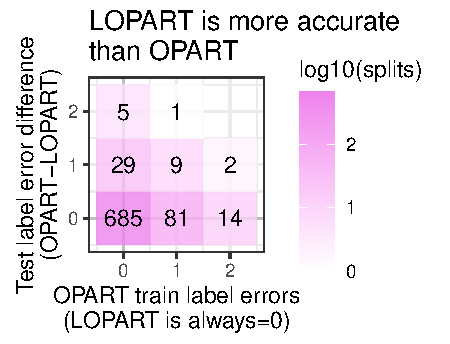
\includegraphics[width=\textwidth]{figure-label-errors}
\end{frame}

\begin{frame}
  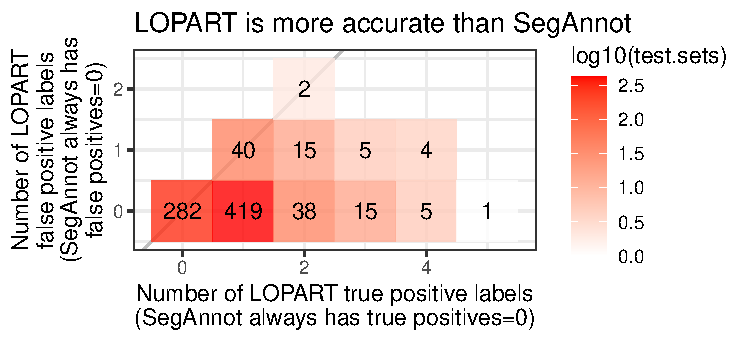
\includegraphics[width=\textwidth]{figure-label-errors-SegAnnot}
\end{frame}

\begin{frame}
  \frametitle{Test accuracy in cross-validation experiments}
  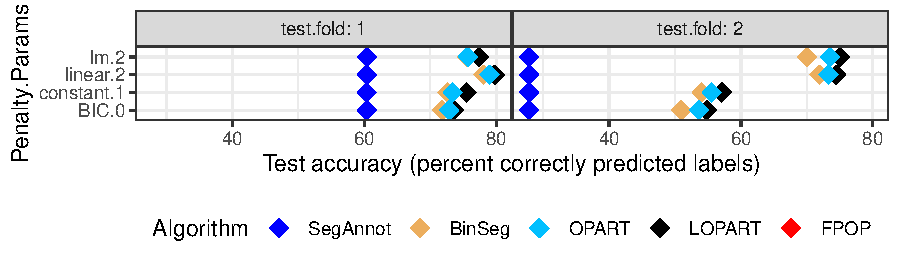
\includegraphics[width=\textwidth]{figure-cv-BIC}
  
\end{frame}

\begin{frame}
  \frametitle{Test ROC curves in cross-validation experiments}
  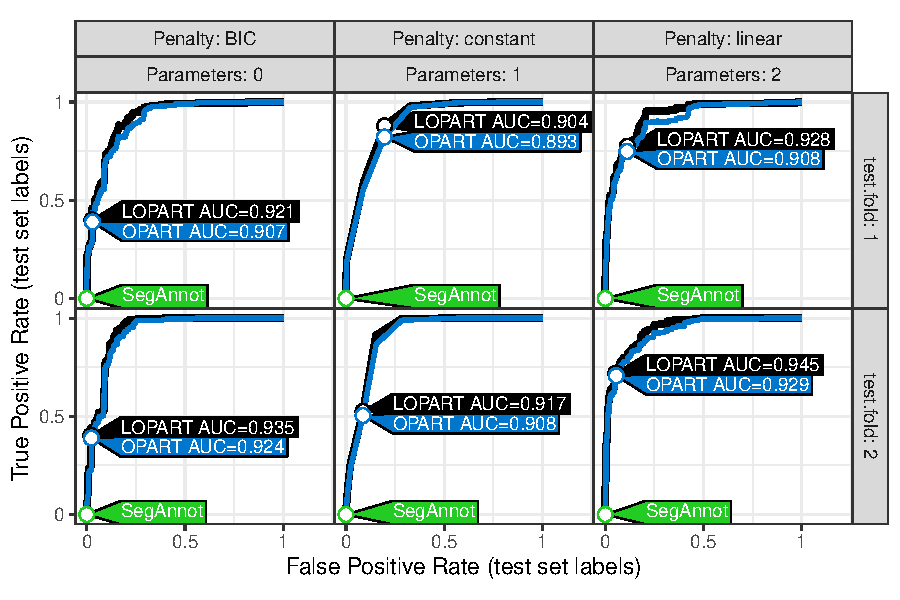
\includegraphics[width=\textwidth]{figure-cv-BIC-roc}
  
\end{frame}

\begin{frame}
  \frametitle{Summary and Discussion}
  \begin{itemize}
  \item Proposed algo fixes issues with two previous algorithms (better
  train AND test accuracy).
\item Results demonstrate improved speed and accuracy.
\item Future work: functional pruning algorithm, which can solve more
  complex constrained changepoint problems (e.g. change must be
  non-decreasing), and should be faster (log-linear instead of
  quadratic).
  \end{itemize}
\end{frame}

\end{document}
